\graphicspath{{images/}}

\section{\thesection~Introduction}
\label{sec:introduction}
Dummy \citet{Lawless2010} citations \citep{Heydari2016} \citep{Addinall2008}.

\subsection{\thesubsection~Subsection}

\begin{Figure}
  \centering
  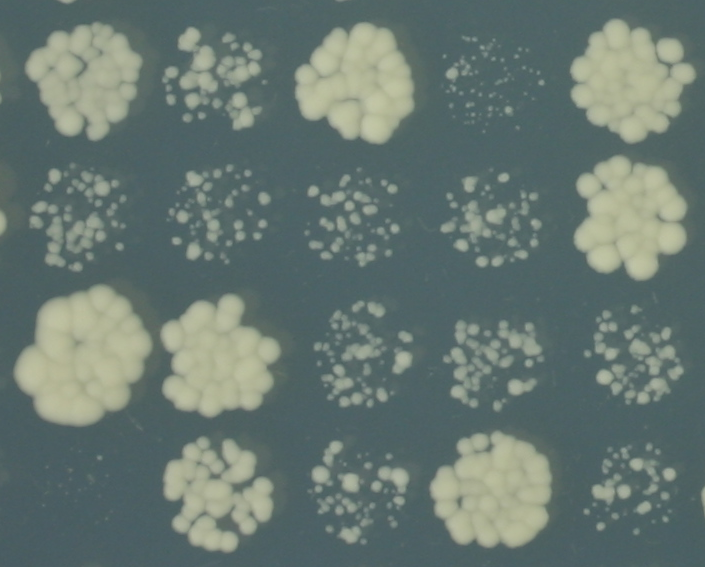
\includegraphics[width=\linewidth]{p15_section/p15_section}
  \captionof{figure}{A section of a plate from a QFA experiment \citep{Addinall2011}.}
  \label{fig:p15_section}
\end{Figure}


\begin{Figure}
  \centering
  \includegraphics[width=\linewidth]{stripes/final/striped}
  \includegraphics[width=\linewidth]{stripes/final/filled}
  \captionof{figure}{Images from an experiment designed to examine
    competition.}
  \label{fig:stripes_images}
\end{Figure}



%%% Local Variables:
%%% mode: latex
%%% TeX-master: "report"
%%% End:
